\chapter{Introduction}
\section{What is OghmaNano?} 
OghmaNano officially stands for \emph{\textbf{O}r\textbf{g}anic and \textbf{h}ybrid \textbf{M}aterial \textbf{N}ano Simulation tool}.  Oghma is also the name of the \href{https://en.wikipedia.org/wiki/Ogma}{Gaelic God} who's appearance is described as "sun-faced" or "shining/radiant", he is creditied with developing \href{https://en.wikipedia.org/wiki/Ogham}{Ogham}, the script in which Irish Gaelic was first written. The creators of OghmaNano spent a lot of time making sure it can describe the light and optical radiation correctly thus the name seems like a good fit. How you remember the name is up to you.

OghmaNano was originally developed to be a general purpose model for simulating photovoltaic devices, including organic and perovskite cells. However, since its initial development the model has expanded to simulate many other classes of optoelectronic devices including, Organic Light Emitting Diodes (OLEDs), Organic Field Effect Transistors (OFETs), large area printed devices, optical filters, photonic crystals and many more.  In general OghmaNano can simulate any opto-electronic-device where electrons, photons (and also heat - phonons) interact.  The model has been downloaded by thousands of people across the globe (see figure \ref{fig:downloadmap}) and is used in many top universities and companies. Figure \ref{fig:alldevices} shows some of the classes of devices OghmaNano can simulate.  Key features of OghmaNano are listed below:

\begin{itemize}
  \item Electrical models:
  \begin{itemize}
    \vspace{-0.2cm}\item 1/2D electrical drift-diffusion solver.
    \vspace{-0.2cm}\item Dynamic SRH traps needed for simulating disordered materials.
    \vspace{-0.2cm}\item Simple equivalent circuit model.
    \vspace{-0.2cm}\item Complex 3D circuit model for complex large area devices.
    \vspace{-0.2cm}\item Arbitrary user defined densities of trap states.
    \vspace{-0.2cm}\item Thermal model linked to the electrical models.
    \vspace{-0.2cm}\item Time domain, frequency domain and steady state solvers.
  \end{itemize}
  \item Optical models:
  \begin{itemize}
    \vspace{-0.2cm}\item Transfer matrix model for light
    \vspace{-0.2cm}\item FDTD models
    \vspace{-0.2cm}\item Ray tracing model
    \vspace{-0.2cm}\item 1/2D optical mode solvers for waveguide structures.
    \vspace{-0.2cm}\item Arbitrary light sources/filters.
  \end{itemize}
  \item Excited states/mobile ion:
  \begin{itemize}
    \vspace{-0.2cm}\item 1/2/3D Exciton solver.
    \vspace{-0.2cm}\item Excited singlet/triplet state solver.
    \vspace{-0.2cm}\item Mobile ions, doping and tunneling through interfaces.
  \end{itemize}
  \item Other/databases:
  \begin{itemize}
    \vspace{-0.2cm}\item Comprehensive materials databases.
    \vspace{-0.2cm}\item Ability to convert arbitrary shapes to 3D objects.
    \vspace{-0.2cm}\item Comprehensive 3D shape database.
  \end{itemize}
\end{itemize}

\section{Why OghmaNano?}
\begin{minipage}{0.5\textwidth}
By burning fossil fuels we are releasing $\sim 33.3$ gigatonnes of $CO_2$ per year \cite{Liu2022} and thus humanity is steadily changing the composition of Earth's atmosphere. Since 1960, $CO_{2}$ in the atmosphere has risen by around \href{https://gml.noaa.gov/ccgg/trends/}{30\%} this in turn is increasing average global temperatures\cite{ManabeandWetherald} and making our home planet Earth, a more difficult place to live on. We therefore have two choices, either cut emissions or face an existential crisis.

Thin film devices such as solar cells and OLEDs offer a viable way to reduce our $CO_{2}$ emissions, either by providing low carbon electricity, or providing an efficient way to use the energy once generated.

\end{minipage}
\hspace{4pt}
\begin{minipage}[]{0.5\linewidth}
\centering
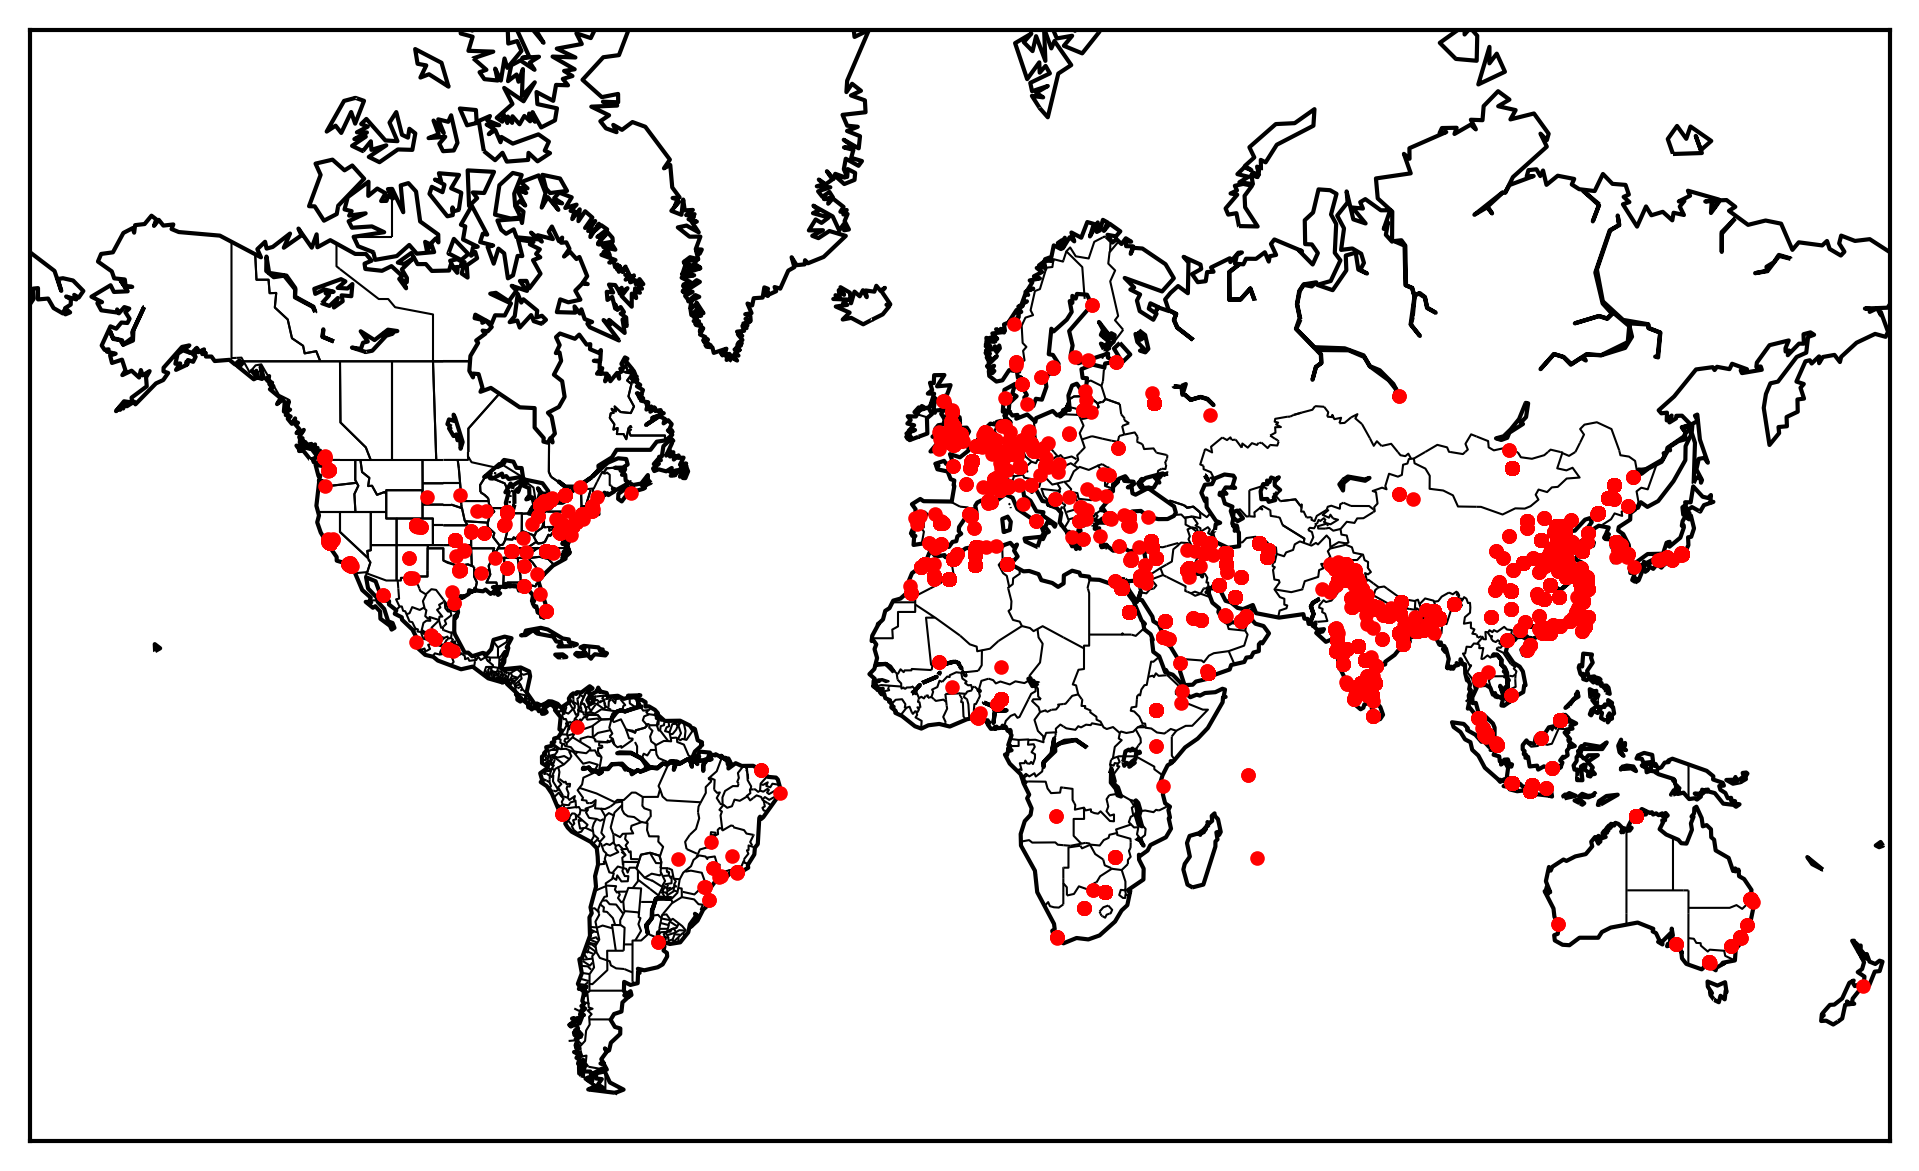
\includegraphics[width=\textwidth]{./images/map.png}
\captionof{figure}{A map of locations where OghmaNano has been downloaded.}
\label{fig:downloadmap}
\end{minipage}

  It is therefore important that technologies based on thin film devices continue to be developed and succeed. By developing and releasing OghmaNano, I hope, I am enabling scientists throughout the world to understand these devices a little bit better, which I hope will contribute in a very small way to solving our climate crisis.

Solar cells and OLEDs happen to come from a class of devices called diodes. This class of devices has many uses including optical sensors, medical sensors, switches, rectifiers. Thus as a pleasant side effect of OghmaNano the development of these devices is also being helped. 

\begin{figure}
\centering
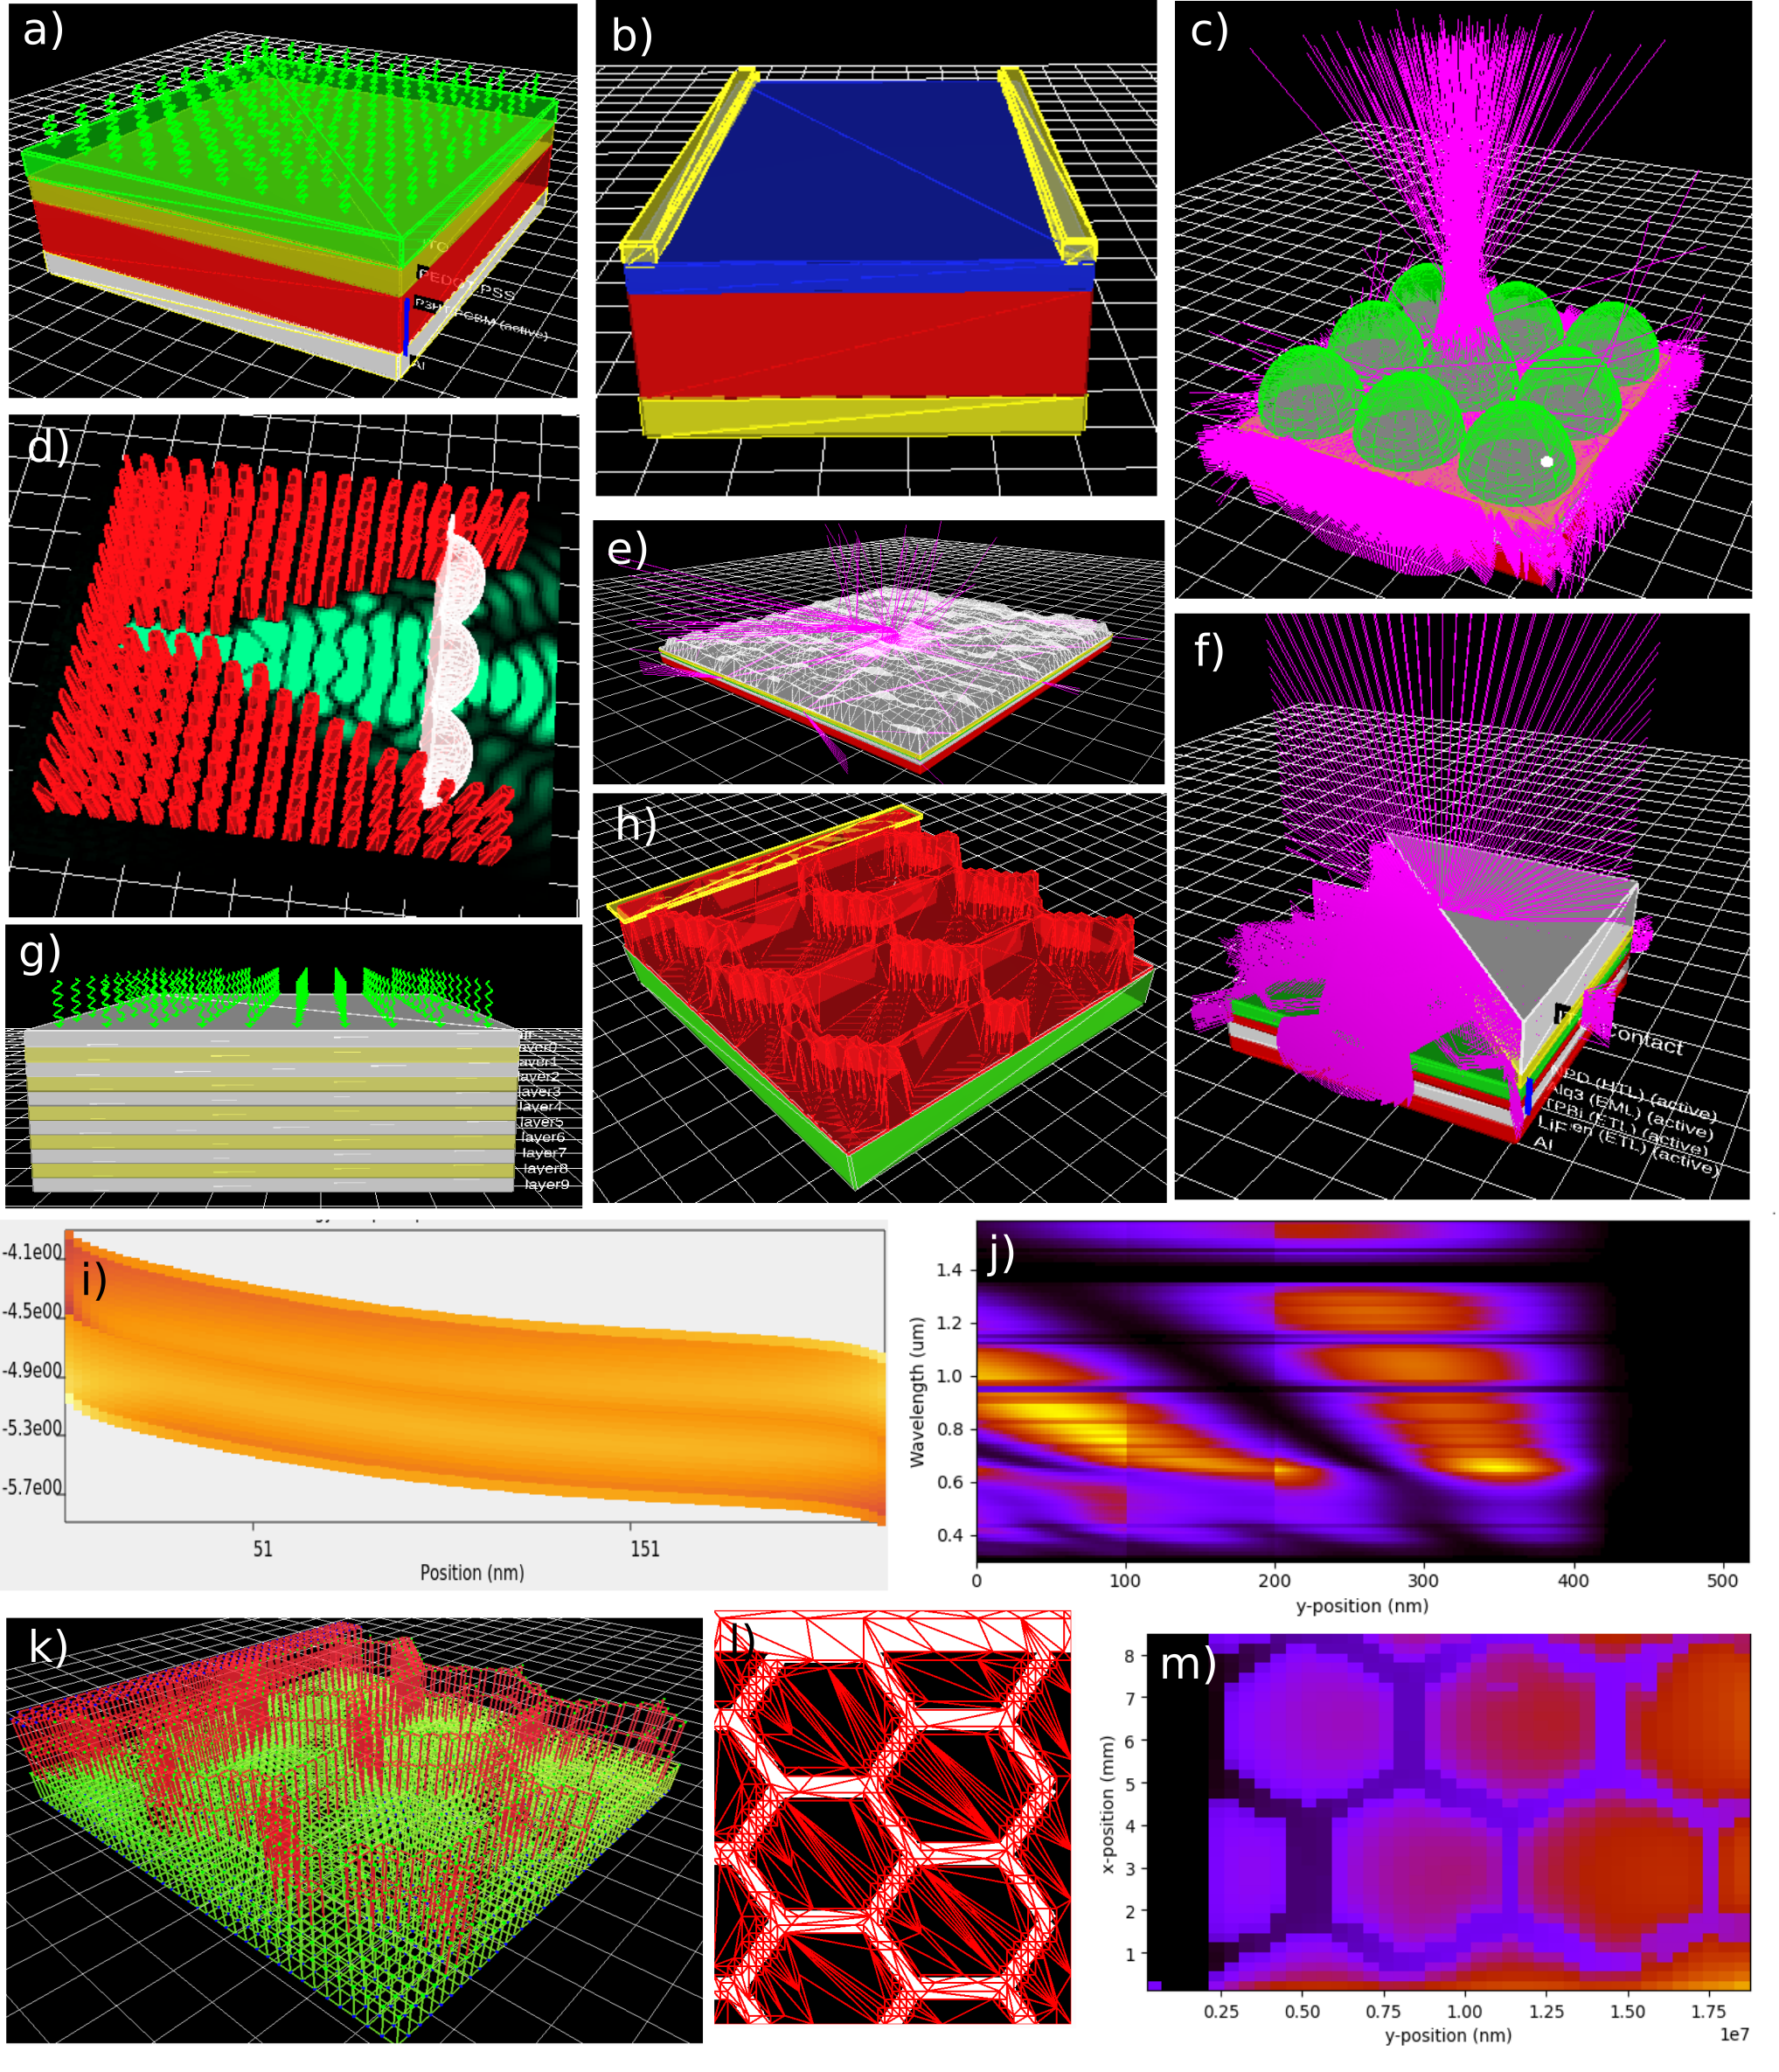
\includegraphics[width=0.9\textwidth]{./images/all_devices.png}
\caption{a); Organic/Perovskite solar cell simulation; b) OFET transistor simulation; c) Microlens simulation; d) Photonic waveguide simulation; e) light escaping structured films; f) OLED simulation; g) Optical filter simulation; h) large area device modelling (hexogonal contacts); i) Mapping carrier density in position/energy space; j) Building complex 3D meshes; and k) resistance maps of large area devices.}
\label{fig:alldevices}
\end{figure}



\section{About this book/manual}
This book is intended to be the definitive guide to simulating devices with OghmaNano. The idea is that one can read this book and learn in a step-by-step way how to simulate many modern opto-electronic devices with very limited prior knolage.  However, not all aspects of this book are yet finished. I therefore recommend you also watch the \href{https://www.youtube.com/channel/UCbm_0AKX1SpbMMT7jilxFfA}{YouTube} channel (and subscribe! ;)) where I describe many of the features in more detail and give demonstrations on the use of the model. I would suggest you treat the videos as lectures (and take notes) rather than entertaining videos (well I hope they are entertaining too!). New releases are generally announced on \href{https://twitter.com/OghmaNano}{Twitter}, which I also suggest you follow to make sure you are using an up-to date version. I often release version every week, a version that is 6 months old is considered very old indeed.  Please read papers which were published from this model - do also read the supplementary information (SI) to the papers, as I often write about the model in there.
This book starts off with explaining how to simulate organic solar cells. This is because organic solar cells are the easiest class of device to simulate, it then moves onto Perovskite devices, and OLEDs. More complex classes of devices follow.  If you are new to simulation work or in indeed OghmaNano, I suggest you start with the first chapters and work your way to the more complex devices.

\section{What is the history of OghmaNano?}
I started writing OghmaNano just after finishing my PhD in 2009 while taking a break for academia and deciding what to do next. At that time it was a simple 1D drift-diffusion diode model designed to simulate solar cells which did not take account of disorder.  Over the next 14 or so years the model has been significantly expanded to model many classes of material system and classes of devices. Since 2009 thousands of people have downloaded OghmaNano and \href{http://www.Oghma-Nano.com/publications.html}{hundreds (the list is by definition always out of date)} of people have published their own papers using the model. If you publish with OghmaNano let me know and I will update the list to include your paper.

\section{What is the roadmap for OghmaNano?}
The aim is to make OghmaNano a completely general opto-electronic model which can be used by anyone to learn about and explore the world of novel opto-electronic devices.  I want OghmaNano to be an engine which people can use to push their own research forward and for education. The exact road map on how to get there is not defined.  As collaborators contact me asking for new features I add them, what comes first depends on what people want.. I never view OghmaNano as finished, and release improvements in small increments, therefore if you discover and report a bug, check back in a week or so to see if it is fixed in the next version.  The same goes for this book, it evolves weekly as I write it. So if a section is missing, check back next week it might be finished.

\section{Using OghmaNano in industrial/academic work}
\label{sec:using_gvpdm}
You are free to use OghmaNano in industrial/academic work. In fact, I'm happy if you do so. However, the following conditions apply:
\begin{enumerate}
  \item If you use OghmaNano to generate results, then clearly say so in your work. This can be as simple as one sentences saying: "we used OghmaNano to perform the simulations"
  \item If you publish a book, paper or thesis where OghmaNano has been used you must cite at least three papers associated with the model.  To find out which papers to cite, click on the area indicated in red in figure \ref{fig:cite_me} when using the model. PLEASE do not cite the manual. I can't include the manual in paper lists when applying for funding.
\end{enumerate}

I ask you to do this because citations are an easy way to demonstrate that people are using OghmaNano. Demonstrating use is key to finding money/people to continue the development of OghmaNano.  So by doing this you are guaranteeing the future of OghmaNano and its continued availability for others.  Thank you!


\begin{figure}
\centering
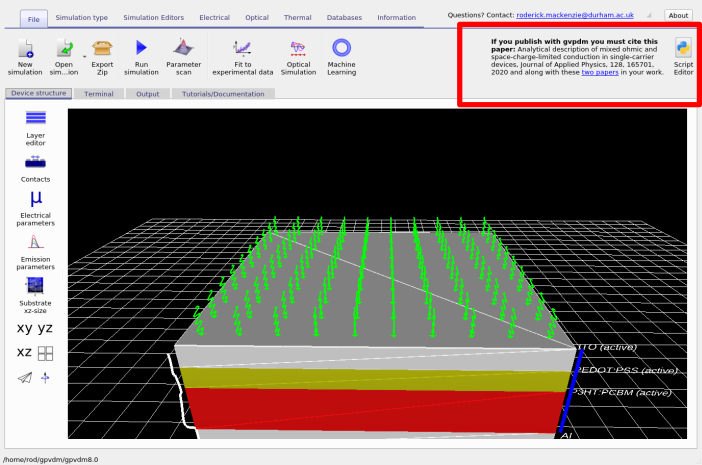
\includegraphics[width=0.7\textwidth]{./images/cite_me2.png}
\caption{If you click on the area indicated by the red box, the model will tell you which papers should be cited.}
\label{fig:cite_me}
\end{figure}

\section{Bugs}
I get quite a lot of feature requests from people wanting features added or for bugs to be fixed. I really appreciate the feedback!  However, I am currently employed at a UK University and my time is split between teaching, research and admin. My performance in my job is measured by the number of high impact papers I push out per year. I therefore have to prioritize feature requests and bug fixes for people who would like to write a paper with me (i.e. my collaborators).... Therefore if you would like:

\begin{itemize}
  \item A bit of advice on how to do x or y with the model then please do feel free to shoot me a mail, and I will do my best to get back to you. If you don't hear back from me just send the mail again.. I get loads of e-mails, and things get lost if I don't answer quickly.
  \item If you want to report a bug, then please do that, and I will do my best to fix it in the next release. But I can't promise when it will be fixed.
  \item  If you would like a features added or a steady stream of help (i.e. you are asking for my time) then please consider inviting me to join in your work and collaborate on a joint paper. I am happy to add whatever feature you want to the model, or fix what ever bug you may have but in return I would ask for the inclusion of my name on the author list. By doing this it makes it much easier for me to justify sinking time into your project.
\end{itemize}
    
If you don't need help from me to use OghmaNano then please feel free to do what you want with the results - no need to contact me, but do cite it correctly.


